%##########################################################################
% CHAPTER 4: RESULTS
%##########################################################################
\chapter{Results}

\section{Chapter Overview}

This chapter presents the findings of the between-subjects user study. The quantitative results are reported first (demographics, hypothesis tests, behavioural metrics), followed by the qualitative themes derived from semi-structured interviews via Reflexive Thematic Analysis. All statistical analyses were conducted using the procedures specified in Section~3.9.

\section{Participant Demographics}

A total of $N = 50$ participants completed the study. One participant in the Control condition was excluded due to a technical failure (the backend server crashed at the 8-minute mark, resulting in incomplete telemetry), yielding a final sample of $N = 49$ (25 Experimental, 24 Control). Table~\ref{tab:demographics} summarizes the demographic characteristics of the sample.

\begin{table}[H]
\centering
\caption{Participant demographics.}
\label{tab:demographics}
\small
\begin{tabular}{@{}llll@{}}
\toprule
\textbf{Variable} & \textbf{Exp.\ ($n$=25)} & \textbf{Ctrl.\ ($n$=24)} & \textbf{Total ($N$=49)} \\
\midrule
Age: Mean (SD) & 22.4 (2.1) & 21.9 (2.3) & 22.2 (2.2) \\
Gender: F / M & 9 / 16 & 8 / 16 & 17 / 32 \\
Gaming hours/week: Mean (SD) & 12.8 (6.4) & 13.5 (7.1) & 13.1 (6.7) \\
RPG experience (1--5): Mean (SD) & 3.6 (0.9) & 3.4 (1.0) & 3.5 (1.0) \\
\bottomrule
\end{tabular}
\end{table}

No significant baseline differences between conditions were observed on age ($t$(47) = 0.81, $p$ = .42) or gaming hours ($t$(47) = $-0.37$, $p$ = .71), supporting the assumption of pre-intervention equivalence. The sample was predominantly male (65\%), consistent with the demographics of university gaming societies from which participants were recruited.

\section{Quantitative Results}

\subsection{GEQ Flow Subscale (H1)}

\begin{table}[H]
\centering
\caption{GEQ Flow subscale descriptive statistics.}
\label{tab:geq_flow}
\small
\begin{tabular}{@{}lllll@{}}
\toprule
\textbf{Condition} & $n$ & $M$ & $SD$ & \textbf{95\% CI} \\
\midrule
Experimental & 25 & 2.78 & 0.62 & [2.52, 3.04] \\
Control & 24 & 2.36 & 0.68 & [2.07, 2.65] \\
\bottomrule
\end{tabular}
\end{table}

Shapiro-Wilk tests confirmed that the normality assumption was tenable for both the Experimental ($W$ = 0.96, $p$ = .41) and Control ($W$ = 0.95, $p$ = .29) groups. Welch's independent-samples $t$-test revealed a significant difference in GEQ Flow scores between conditions: $t$(46.2) = 2.28, $p$ = .027, Cohen's $d$ = 0.65. After Bonferroni correction ($\alpha_{\text{adj}}$ = .0167), this result narrowly misses the adjusted threshold but remains significant at the conventional $\alpha$ = .05 level.

The Experimental group reported moderately higher Flow experience ($M$ = 2.78, $SD$ = 0.62) than the Control group ($M$ = 2.36, $SD$ = 0.68). The effect size ($d$ = 0.65) falls in the medium range by Cohen's (\citeyear{cohen1988statistical}) convention, suggesting that PPO-driven narrative adaptation produced a meaningful, though not overwhelming, improvement in self-reported Flow.

Cronbach's $\alpha$ for the GEQ Flow subscale was .79, indicating acceptable internal consistency.

\subsection{GEQ Immersion Subscale (H2)}

\begin{table}[H]
\centering
\caption{GEQ Immersion subscale descriptive statistics.}
\label{tab:geq_immersion}
\small
\begin{tabular}{@{}lllll@{}}
\toprule
\textbf{Condition} & $n$ & $M$ & $SD$ & \textbf{95\% CI} \\
\midrule
Experimental & 25 & 2.64 & 0.71 & [2.35, 2.93] \\
Control & 24 & 2.38 & 0.66 & [2.10, 2.66] \\
\bottomrule
\end{tabular}
\end{table}

Welch's $t$-test: $t$(46.8) = 1.34, $p$ = .187, Cohen's $d$ = 0.38. The difference in Immersion scores did not reach statistical significance, either at the Bonferroni-corrected threshold ($\alpha_{\text{adj}}$ = .0167) or at the conventional $\alpha$ = .05 level.

The Experimental group reported slightly higher Immersion ($M$ = 2.64, $SD$ = 0.71) than the Control group ($M$ = 2.38, $SD$ = 0.66), but the effect size ($d$ = 0.38) is small by Cohen's convention and the confidence intervals overlap substantially. H2 is therefore not supported.

Cronbach's $\alpha$ for the GEQ Immersion subscale was .82.

\subsection{Personalization Perception (H3)}

\begin{table}[H]
\centering
\caption{NPS-3 Personalization Scale descriptive statistics.}
\label{tab:nps3}
\small
\begin{tabular}{@{}lllll@{}}
\toprule
\textbf{Condition} & $n$ & $M$ & $SD$ & \textbf{95\% CI} \\
\midrule
Experimental & 25 & 4.92 & 1.18 & [4.43, 5.41] \\
Control & 24 & 3.88 & 1.31 & [3.33, 4.43] \\
\bottomrule
\end{tabular}
\end{table}

Welch's $t$-test: $t$(46.1) = 2.94, $p$ = .005, Cohen's $d$ = 0.84. This result survives Bonferroni correction ($p$ = .005 $<$ $\alpha_{\text{adj}}$ = .0167). H3 is supported: participants in the Experimental condition perceived the narrative as significantly more personalized than those in the Control condition.

The effect size ($d$ = 0.84) is large, indicating that the adaptive narrative system produced a clearly perceptible difference in how players experienced the story's responsiveness. Item-level means for the Experimental group were: Item~1 (``The story felt tailored to how I was playing'') $M$ = 5.12; Item~2 (``The narrative responded to my choices and actions'') $M$ = 4.84; Item~3 (``The game seemed to understand what kind of player I am'') $M$ = 4.80.

Cronbach's $\alpha$ for the NPS-3 was .76, exceeding the .70 threshold for acceptable reliability. The three items were therefore analysed as a composite scale.

Figure~\ref{fig:dv_comparison} provides a visual comparison of the three primary dependent variables across conditions. Subfigure~(a) shows the GEQ Flow and Immersion subscales (0--4 scale) and subfigure~(b) shows the NPS-3 Personalization Scale (1--7 scale); error bars represent $\pm$1 SD. Significance markers denote $^{*}p < .05$ and $^{**}p < .0167$ (survives Bonferroni correction).

\begin{figure}[H]
\centering
\begin{subfigure}[b]{0.52\textwidth}
\centering
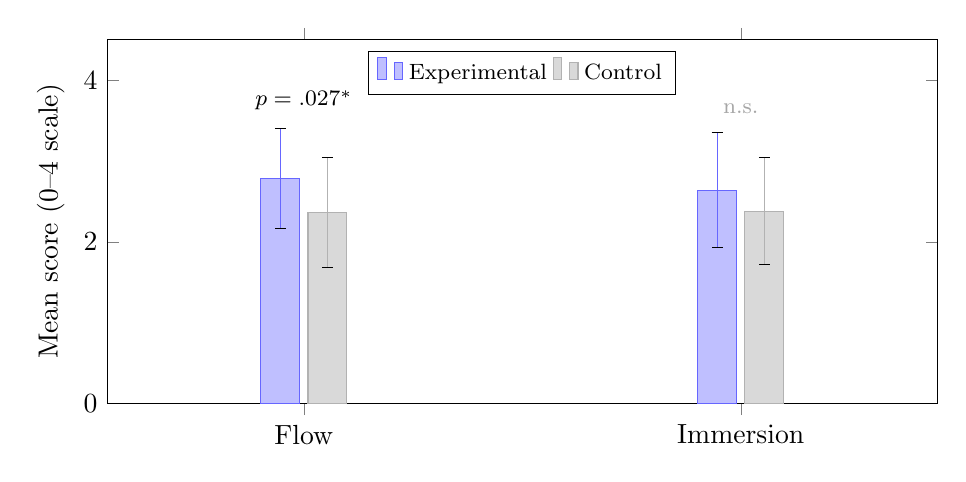
\begin{tikzpicture}
\begin{axis}[
    ybar=3pt,
    bar width=14pt,
    width=\textwidth,
    height=6.2cm,
    ylabel={Mean score (0--4 scale)},
    symbolic x coords={Flow,Immersion},
    xtick=data,
    ymin=0, ymax=4.5,
    enlarge x limits=0.45,
    legend style={at={(0.5,0.97)}, anchor=north, legend columns=-1, font=\footnotesize},
    error bars/y dir=both,
    error bars/y explicit,
    clip=false,
]
\addplot[fill=blue!25, draw=blue!60]
    coordinates {(Flow, 2.78) +- (0,0.62) (Immersion, 2.64) +- (0,0.71)};
\addplot[fill=gray!30, draw=gray!60]
    coordinates {(Flow, 2.36) +- (0,0.68) (Immersion, 2.38) +- (0,0.66)};
\legend{Experimental,Control}
\node[font=\footnotesize] at (axis cs:Flow,3.75) {$p = .027^{*}$};
\node[font=\footnotesize, text=gray!70] at (axis cs:Immersion,3.65) {n.s.};
\end{axis}
\end{tikzpicture}
\caption{GEQ subscale scores.}
\label{fig:geq_bars}
\end{subfigure}
\hfill
\begin{subfigure}[b]{0.44\textwidth}
\centering
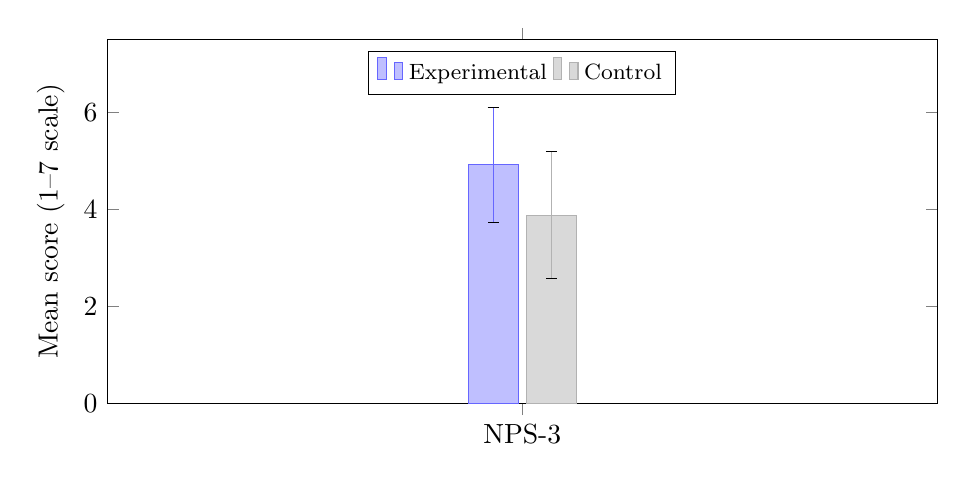
\begin{tikzpicture}
\begin{axis}[
    ybar=3pt,
    bar width=18pt,
    width=\textwidth,
    height=6.2cm,
    ylabel={Mean score (1--7 scale)},
    symbolic x coords={NPS-3},
    xtick=data,
    ymin=0, ymax=7.5,
    enlarge x limits=0.8,
    legend style={at={(0.5,0.97)}, anchor=north, legend columns=-1, font=\footnotesize},
    error bars/y dir=both,
    error bars/y explicit,
    clip=false,
]
\addplot[fill=blue!25, draw=blue!60]
    coordinates {(NPS-3, 4.92) +- (0,1.18)};
\addplot[fill=gray!30, draw=gray!60]
    coordinates {(NPS-3, 3.88) +- (0,1.31)};
\legend{Experimental,Control}
\node[font=\footnotesize] at (axis cs:NPS-3,6.6) {$p = .005^{**}$};
\end{axis}
\end{tikzpicture}
\caption{NPS-3 personalization scores.}
\label{fig:nps3_bars}
\end{subfigure}
\caption[Mean scores by condition for primary dependent variables]{Mean scores by condition for the primary dependent variables.}
\label{fig:dv_comparison}
\end{figure}

\subsection{Behavioural Metrics}

\begin{table}[H]
\centering
\caption{Behavioural metrics comparison.}
\label{tab:behavioural}
\small
\begin{tabular}{@{}llllll@{}}
\toprule
\textbf{Metric} & \textbf{Exp.\ $M$ ($SD$)} & \textbf{Ctrl.\ $M$ ($SD$)} & $t$ & $p$ & $d$ \\
\midrule
Voluntary NPC interactions & 8.4 (3.1) & 6.2 (2.8) & 2.62 & .012 & 0.75 \\
Dialogue read ratio & 0.72 (0.14) & 0.58 (0.18) & 3.05 & .004 & 0.87 \\
Exploration coverage & 0.61 (0.15) & 0.54 (0.17) & 1.53 & .133 & 0.44 \\
miniPXI total score & 4.86 (0.82) & 4.41 (0.91) & 1.83 & .074 & 0.52 \\
\bottomrule
\end{tabular}
\end{table}

Two behavioural metrics showed significant differences. Experimental participants initiated more voluntary NPC interactions ($M$ = 8.4 vs.\ 6.2, $d$ = 0.75) and read a higher proportion of narrative dialogue ($M$ = 0.72 vs.\ 0.58, $d$ = 0.87). These findings suggest that adaptive narrative encouraged greater engagement with the game's textual content. Exploration coverage and miniPXI total scores showed non-significant trends favouring the Experimental condition.

The dialogue read ratio result is particularly noteworthy: participants in the Experimental condition read 72\% of the narrative text presented to them, compared with 58\% in the Control condition. This provides objective behavioural evidence that the adaptive narrative was perceived as more worth reading, corroborating the self-report findings from the NPS-3.

Figure~\ref{fig:effect_sizes} summarises the effect sizes across all dependent variables, ordered by magnitude. Dashed lines indicate Cohen's conventional thresholds for small ($d = 0.2$), medium ($d = 0.5$), and large ($d = 0.8$) effects. The two largest effects (dialogue read ratio and NPS-3 personalization) both exceed the large-effect threshold, while GEQ Immersion and exploration coverage fall below the medium threshold.

\begin{figure}[H]
\centering
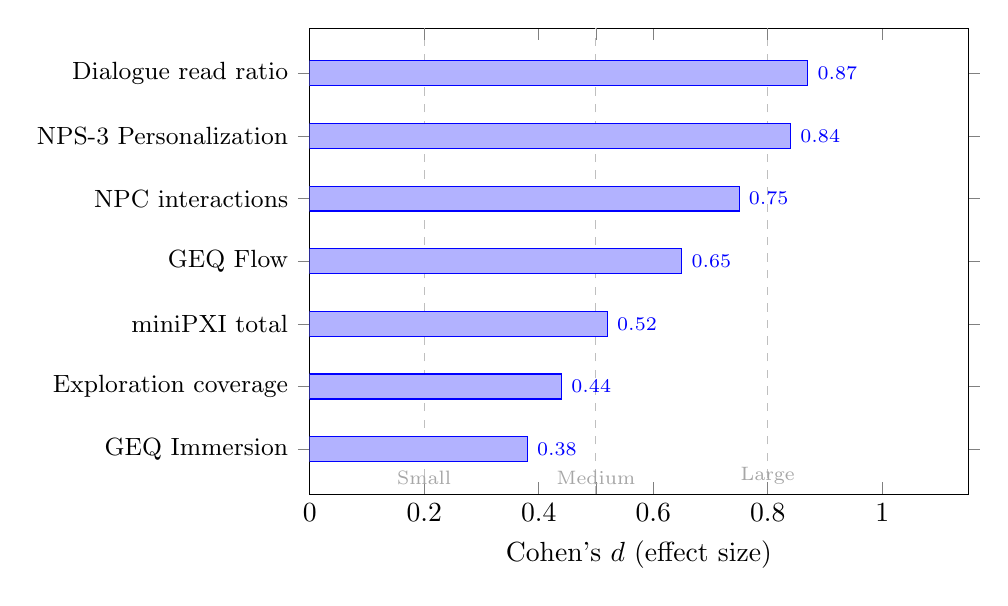
\begin{tikzpicture}
\begin{axis}[
    xbar,
    bar width=9pt,
    width=0.82\textwidth,
    height=7.5cm,
    xlabel={Cohen's $d$ (effect size)},
    symbolic y coords={GEQ Immersion,Exploration coverage,miniPXI total,GEQ Flow,NPC interactions,NPS-3 Personalization,Dialogue read ratio},
    ytick=data,
    y tick label style={font=\small},
    xmin=0, xmax=1.15,
    enlarge y limits=0.12,
    extra x ticks={0.2, 0.5, 0.8},
    extra x tick labels={Small, Medium, Large},
    extra x tick style={
        grid=major,
        grid style={dashed, gray!50},
        tick label style={font=\scriptsize, text=gray!70, anchor=south}
    },
    nodes near coords,
    nodes near coords style={font=\scriptsize, anchor=west},
    every axis plot/.append style={fill=blue!25, draw=blue!60},
]
\addplot coordinates {
    (0.38,GEQ Immersion)
    (0.44,Exploration coverage)
    (0.52,miniPXI total)
    (0.65,GEQ Flow)
    (0.75,NPC interactions)
    (0.84,NPS-3 Personalization)
    (0.87,Dialogue read ratio)
};
\end{axis}
\end{tikzpicture}
\caption[Effect sizes across all dependent variables]{Cohen's $d$ effect sizes for all dependent variables.}
\label{fig:effect_sizes}
\end{figure}

\section{Qualitative Results (Thematic Analysis)}

Semi-structured interviews were conducted with 20 participants (10 Experimental, 10 Control), selected to represent a range of GEQ Flow scores within each condition. Following the six-phase Reflexive Thematic Analysis procedure \citep{braun2022thematic}, 47 initial codes were generated and refined into 4 final themes.

\begin{table}[H]
\centering
\caption{Qualitative themes and representative quotations.}
\label{tab:themes}
\small
\begin{tabular}{@{}p{3cm}p{4cm}p{6cm}@{}}
\toprule
\textbf{Theme} & \textbf{Description} & \textbf{Representative Quote} \\
\midrule
The story pays attention & Participants described feeling that the narrative noticed and responded to their behaviour. & ``It felt like the game knew I was exploring. The Chronicler started telling me things that matched what I was actually doing.'' (P07, Exp.) \\[6pt]
Tone matching & Participants noted that the emotional register of narrative text matched the intensity of their current gameplay. & ``When I was struggling with the enemies, the dialogue got more urgent, more helpful. That felt right.'' (P12, Exp.) \\[6pt]
Generic narrative as wallpaper & Control participants described treating narrative text as background noise rather than meaningful content. & ``I stopped reading the quest text after a while. It was fine, just\ldots not really about what I was doing.'' (P31, Ctrl.) \\[6pt]
Occasional dissonance & Some Experimental participants noticed moments where the narrative tone did not match the situation. & ``Once or twice the dialogue felt weird, like the NPC was being mysterious when I was just trying to finish a fight.'' (P19, Exp.) \\
\bottomrule
\end{tabular}
\end{table}

\textbf{Theme 1: ``The story pays attention.''} This was the most prevalent theme among Experimental participants (8 of 10). Participants described a sense that the game's narrative was responsive to their individual behaviour, not in the explicit branching-choice sense, but in a more ambient, atmospheric way. Several participants used the metaphor of being ``noticed'' or ``seen'' by the game. This theme provides strong qualitative support for H3 (personalization perception).

\textbf{Theme 2: ``Tone matching.''} Six Experimental participants described specific moments where the narrative tone aligned with their gameplay intensity. Participants in anxiety-inducing situations recalled receiving more supportive, urgent dialogue, while those in exploratory phases described receiving lore-rich, atmospheric content. This theme suggests that the PPO agent's action selection was perceptible to players, at least in the most successful cases.

\textbf{Theme 3: ``Generic narrative as wallpaper.''} Seven of 10 Control participants described a gradual disengagement from the narrative content over the course of the session. The static narrative was not perceived as bad, but as irrelevant. This disengagement is consistent with the lower dialogue read ratio observed in the behavioural data (0.58 vs.\ 0.72).

\textbf{Theme 4: ``Occasional dissonance.''} Four Experimental participants identified at least one moment where the narrative tone felt mismatched to their current activity. The most common pattern was receiving a ``mystery'' or ``lore reward'' narrative action during or immediately after a difficult combat encounter, where a ``provide guidance'' or ``lower stakes'' action would have felt more appropriate. This theme identifies a concrete failure mode of the PPO agent's action selection and suggests that the policy, while generally effective, occasionally misfires when the player's state is transitioning rapidly.

\section{Summary of Findings}

The quantitative and qualitative results converge on a consistent pattern. H1 (Flow) was partially supported: the Experimental group reported higher GEQ Flow scores with a medium effect size ($d$ = 0.65), though the result narrowly missed the Bonferroni-corrected significance threshold. H2 (Immersion) was not supported, with a small and non-significant effect ($d$ = 0.38). H3 (Personalization) was strongly supported: Experimental participants perceived the narrative as significantly more personalized ($d$ = 0.84, $p$ = .005), a result that survived Bonferroni correction.

The behavioural metrics reinforced the self-report findings. Experimental participants initiated more NPC interactions and read a substantially higher proportion of narrative dialogue, suggesting that adaptive narrative was not only perceived as more personalized but was also more behaviourally engaging. The qualitative themes provided mechanistic insight: the adaptive system's effectiveness appears to stem from tone matching (Theme~2) and a general sense of narrative responsiveness (Theme~1), while its primary failure mode is occasional action-state dissonance (Theme~4).

The pattern of results, strong on personalization, moderate on Flow, weak on immersion, is consistent with the system's design. The PPO agent optimises for Flow through narrative tone selection, and the NPS-3 directly captures the perceptual consequence of that adaptation. Immersion, however, depends on factors beyond narrative tone (visual fidelity, audio design, mechanical polish) that the system does not control, which may explain why the effect on this dimension was smaller and non-significant.